% Created 2024-03-03 Sun 20:59
% Intended LaTeX compiler: pdflatex
\documentclass[11pt,oneside]{memoir}
\makeatletter

\usepackage{answerkey-env}

\ifanswerkey
  \usepackage[forcolorpaper, answerkey]{eqexam}
  \usepackage{vinaya-class-questions}
\else
  \usepackage[forcolorpaper, nosolutions]{eqexam}
  \usepackage[nosolutions]{vinaya-class-questions}
\fi

\proofingsymbolColor{linkred}
\fillinColor{linkred}

\def\maketitle{}

\maxtocdepth{subsection}

\newenvironment{twocols}{%
  \raggedright%
  \setlength{\parindent}{0pt}%
  \setlength{\parskip}{8pt}%
  \fontsize{11}{17}\selectfont%
  \begin{multicols}{2}%
}{%
  \end{multicols}%
}

\newenvironment{widecols}{%
  \hspace*{-0.05\linewidth}\begin{minipage}{1.1\linewidth}%
  \raggedright%
  \setlength{\parindent}{0pt}%
  \setlength{\parskip}{8pt}%
  \fontsize{11}{17}\selectfont%
  \begin{multicols}{2}%
}{%
  \end{multicols}%
  \end{minipage}%
}

\newlength\@tmp@width
\newlength\@tmp@height

\renewcommand*{\printchaptertitleHook}{%
  \AddToShipoutPictureBG*{%
    \put(\LenToUnit{\paperwidth-25mm-\spinemargin},\LenToUnit{\paperheight-95mm}){%
      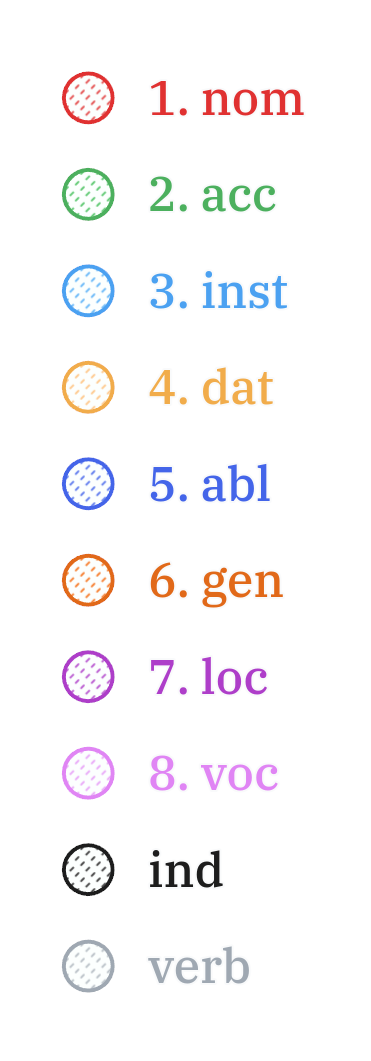
\includegraphics[width=25mm]{./images/cases-legend-white-large.png}%
    }%
  }%
}

\newcommand*\sentenceDiaMsg{\textbf{Exercise:} Draw a sentence analysis diagram below and indicate declensions.}

\newcommand*\sentenceDiaSolution[2][0.4]{%
  \ifanswerkey%
    \hspace*{-\spinemargin}%
    \begin{minipage}{\paperwidth}%
      \centering%
      \includegraphics[scale=#1]{#2}%
    \end{minipage}%
  \else%
    \settototalheight{\@tmp@height}{\includegraphics[scale=#1]{#2}}%
    \begin{minipage}[\@tmp@height]{\linewidth}%
      \sentenceDiaMsg%
    \end{minipage}%
  \fi%
}

\usepackage{cwpuzzle}

\renewcommand\PuzzleCluePre{%
  \begin{minipage}[t]{0.75\linewidth}%
}

\renewcommand\PuzzleClueFont{\fontsize{11}{17}\selectfont}

% \def\PuzzleThickline{\linethickness{2pt}}

\makeatother

\maxtocdepth{section}
\date{\today}
\title{Pali Readings with Sentence Analysis}
\hypersetup{
 pdfauthor={The Bhikkhu Saṅgha},
 pdftitle={Pali Readings with Sentence Analysis},
 pdfkeywords={},
 pdfsubject={},
 pdfcreator={Emacs 29.2 (Org mode 9.6.15)}, 
 pdflang={En_Gb}}
\begin{document}

\maketitle
\frontmatter

{\centering

{\Huge Pāḷi Readings with Sentence Analysis}

\bigskip
\href{https://vinaya-class.github.io}{https://vinaya-class.github.io}

{\scshape\small last updated on}\\
\today

}

\bigskip
\tableofcontents*

\mainmatter

\yournamefalse

\newlength{\colOne}\setlength{\colOne}{0.35\linewidth}
\newlength{\colTwo}\setlength{\colTwo}{0.6\linewidth}

\renewenvironment{quote}%
{\list{}{%
    \doubleLineSize
    \listparindent 0pt
    \itemindent    0pt
    \leftmargin    3em
    \rightmargin   3em
    \parsep        0pt
    \topsep        8pt
    \partopsep     0pt}%
\item[] \raggedright}%
{\endlist}

\chapter{The Weaver's Daughter (Dhp 174 and Comm.)}
\label{sec:orgb4aa596}
\section{Sā olokitasaññāṇeneva\ldots{}}
\label{sec:org4511d85}

\begin{quote}
Sā olokitasaññāṇeneva satthāraṁ upasaṅkamitvā

chabbaṇṇaraṁsīnaṁ antaraṁ pavisitvā vanditvā ekamantaṁ aṭṭhāsi.

Tathārūpāya parisāya majjhe nisīditvā

tuṇhībhūtaṁ satthāraṁ vanditvā ṭhitakkhaṇeyeva taṁ āha –
\end{quote}

\begin{longtable}{L{\colOne} L{\colTwo} H}
olokita (pp.) & being looked at & Sā \{\{olokita\}\}saññāṇeneva satthāraṁ upasaṅkamitvā\\[0pt]
saññāṇa (nt.) & mental noting; lit. marking & Sā olokita\{\{saññāṇe\}\}neva satthāraṁ upasaṅkamitvā\\[0pt]
chabbaṇṇaraṁsi (f.) & six-coloured light-ray & \{\{chabbaṇṇaraṁsīnaṁ\}\} antaraṁ pavisitvā\\[0pt]
antaraṁ (ind.) & inside; near to; across; in the vicinity of & chabbaṇṇaraṁsīnaṁ \{\{antaraṁ\}\} pavisitvā\\[0pt]
aṭṭhāsi & stood (aor.2nd/3rd. of tiṭṭhati) & pavisitvā vanditvā ekamantaṁ \{\{aṭṭhāsi\}\}\\[0pt]
parisā (f.) & assembly; meeting; forum; gathering; group & Tathārūpāya \{\{parisāya\}\} majjhe nisīditvā\\[0pt]
tuṇhībhūta (pp.) & silent; quiet; mute & \{\{tuṇhībhūtaṁ\}\} satthāraṁ vanditvā\\[0pt]
khaṇa (m.) & moment; instant; point in time; opportunity & ṭhita\{\{kkhaṇe\}\}yeva taṁ āha\\[0pt]
\end{longtable}

\enlargethispage{\baselineskip}
\sentenceDiaSolution{./images/dhp174-sa-olokita.png}

\clearpage

\begin{quote}
'kumārike, kuto āgacchasī'ti? 'na jānāmi, bhante'ti.

'kattha gamissasī'ti? 'na jānāmi, bhante'ti.

'na jānāsī'ti? 'jānāmi, bhante'ti.

'jānāsī'ti? 'na jānāmi, bhante'ti.

Iti naṁ satthā cattāro pañhe pucchi.
\end{quote}

\begin{longtable}{L{\colOne} L{\colTwo} H}
kuto (ind.) & from where? [ka + to] & Kumārike, \{\{kuto\}\} āgacchasi?\\[0pt]
kattha (ind.) & where? [ka + ttha] & \{\{Kattha\}\} gamissasi?\\[0pt]
naṁ (pron.) & him, her, it (nt.acc.sg. of ta) & Iti \{\{naṁ\}\} satthā cattāro pañhe pucchi.\\[0pt]
\end{longtable}

\sentenceDiaSolution{./images/dhp174-kumarike-kuto.png}

\clearpage

\begin{quote}
Mahājano ujjhāyi -- 'ambho, passatha,

Ayaṁ pesakāradhītā sammāsambuddhena saddhiṁ icchiticchitaṁ kathesi,

nanu nāma imāya 'Kuto āgacchasī'ti vutte

'Pesakāragehato'ti vattabbaṁ.

'Kahaṁ gacchasī'ti vutte

'Pesakārasāla'nti vattabbaṁ siyā'ti.
\end{quote}

\begin{longtable}{L{\colOne} L{\colTwo} H}
ujjhāyi & complained; grumbled (about); lit. thought down (aor. of \emph{ujjhayati}) & Mahājano \{\{ujjhāyi\}\}\\[0pt]
ambho (ind.) & Hey! Look here! & \\[0pt]
icchiticchita & whatever one wishes; whichever desired; [icchita + icchita] & Ayaṁ pesakāradhītā sammāsambuddhena saddhiṁ \{\{icchiticchitaṁ\}\} kathesi\\[0pt]
nanu nāma & surely certainly & \\[0pt]
vutta (pp.) & said; told; spoken; mentioned & imāya 'Kuto āgacchasī'ti \{\{vutte\}\}\\[0pt]
kahaṁ (ind.) & where? [ka + haṁ] & \\[0pt]
siyā & could be; may be; might be; should be (opt. of \emph{atthi}, irreg) & 'Pesakārasāla'nti vattabbaṁ \{\{siyā\}\}.\\[0pt]
\end{longtable}

\sentenceDiaSolution{./images/dhp174-mahajano-ujjhayi.png}

\clearpage

\begin{quote}
Satthā mahājanaṁ nissaddaṁ katvā,

'Kumārike, tvaṁ kuto āgacchasī'ti vutte

'Kasmā na jānāmīti vadesī'ti pucchi.
\end{quote}

\begin{longtable}{L{\colOne} L{\colTwo} H}
nissadda (adj.) & silent, noiseless [nis + sadda] & Satthā mahājanaṁ \{\{nissaddaṁ\}\} katvā\\[0pt]
\end{longtable}

\sentenceDiaSolution{./images/dhp174-sattha-mahajanam.png}

\clearpage

\begin{quote}
Bhante, tumhe mama pesakāragehato āgatabhāvaṁ jānātha,

'Kuto āgatāsī'ti pucchantā pana

'Kuto āgantvā idha nibbattāsī'ti pucchatha.

Ahaṁ pana na jānāmi 'Kuto ca āgantvā idha nibbattāmhī'ti.

Athassā satthā 'Sādhu sādhu, kumārike,

mayā pucchitapañhova tayā vissajjito'ti
\end{quote}

\begin{longtable}{L{\colOne} L{\colTwo} H}
āgatabhāva & came to be (in this state) [āgata + bhāva] & mama pesakāragehato \{\{āgatabhāvaṁ\}\}\\[0pt]
nibbatta (pp.) & arisen from; reborn from; lit. come out [nī + √vatt + ta] & Kuto āgantvā idha \{\{nibbatt\}\}āsi?\\[0pt]
asi (pr.) & you are (pr.2nd.sg. of \emph{atthi}) & Kuto āgantvā idha nibbatt\{\{āsi\}\}?\\[0pt]
\end{longtable}

\sentenceDiaSolution{./images/dhp174-mama-pesakaragehato.png}

\clearpage

\begin{quote}
Paṭhamaṁ sādhukāraṁ datvā uttarimpi pucchi --

'Kattha gamissasīti puna puṭṭhā kasmā `na jānāmī'ti vadesī'ti?

Bhante, tumhe maṁ tasarapacchiṁ gahetvā

pesakārasālaṁ gacchantiṁ jānātha,

'ito gantvā kattha nibbattissasī'ti pucchatha.
\end{quote}

\begin{longtable}{L{\colOne} L{\colTwo} H}
sādhukāra (m.) & applause; approval; cheering; well wishing & Paṭhamaṁ \{\{sādhukāraṁ\}\} datvā uttarimpi pucchi\\[0pt]
uttari (ind.) & furthermore; what is more; moreover & Paṭhamaṁ sādhukāraṁ datvā \{\{uttarimpi\}\} pucchi\\[0pt]
\end{longtable}

\sentenceDiaSolution{./images/dhp174-pathamam-sadhukaram.png}

\clearpage

\begin{quote}
Ahañca ito cutā na jānāmi 'kattha gantvā nibbattissāmī'ti.

Athassā satthā 'mayā pucchitapañhoyeva tayā vissajjito'ti
\end{quote}

\begin{longtable}{L{\colOne} L{\colTwo} H}
cuta (pp.) & passed away; died (pp. of \emph{cavati}) & Ahañca ito \{\{cutā\}\} na jānāmi\ldots{}\\[0pt]
\end{longtable}

\sentenceDiaSolution{./images/dhp174-ito-cuta.png}
\end{document}
